\documentclass[t]{beamer}
%\usetheme{amcg}
\usetheme{iclpt}

\usepackage{color,listings}
\usepackage{pstricks, pst-node}
\usepackage{pgfpages,xspace,array}

\newcommand{\doc}[1]{\psshadowbox[framearc=0]{#1}}
\newcommand{\program}[1]{\psframebox[framearc=.2]{#1}}

\usepackage{graphicx,stmaryrd,cancel}
\usepackage{bibentry}
\usepackage{hyperref}
\usepackage{amscd}
\usepackage{booktabs}
\bibliographystyle{elsarticle-harv}

\expandafter\ifx\csname natexlab\endcsname\relax\def\natexlab#1{#1}\fi
\expandafter\ifx\csname url\endcsname\relax
  \def\url#1{\texttt{#1}}\fi
\expandafter\ifx\csname urlprefix\endcsname\relax\def\urlprefix{URL }\fi

\definecolor{icdarkblue}{RGB}{23,18,134}
\definecolor{icdarkgreen}{RGB}{0,130,0}

%\setbeameroption{show notes on second screen}

\author[David A. Ham]{Dr David~A.~Ham BSc LLB} 
\date{24 May 2013}

\title{Principles of copyright in software}
                  
\institute[Imperial College London]{
  Department of Computing, Imperial College London\\
david.ham@imperial.ac.uk}

\begin{document}
\nobibliography{bibliography}

\begin{frame}[plain]
  \vfill{}

  \centering

  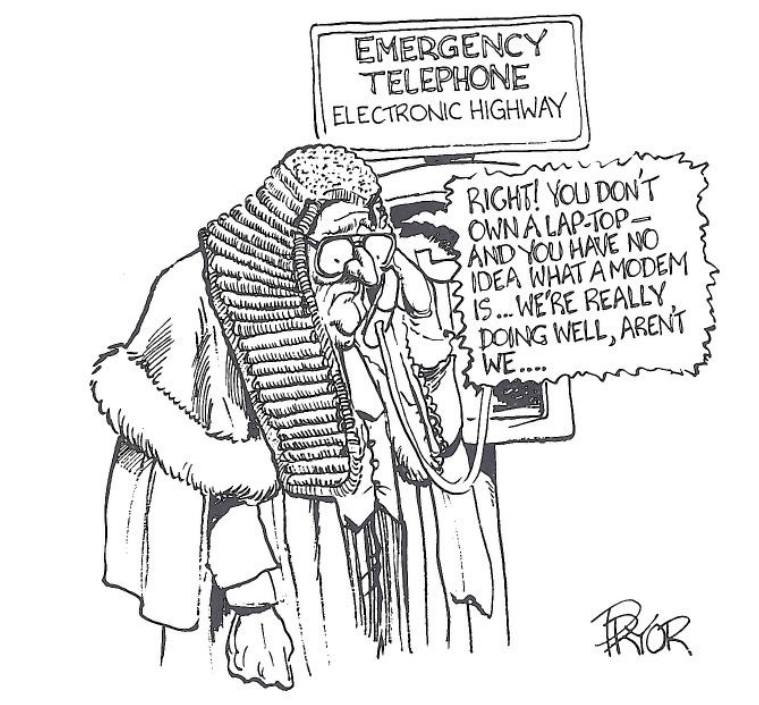
\includegraphics[height=.8\textheight]{judge.png}

  \Large\color{icdarkblue}\inserttitle\\
  %\normalsize\insertsubtitle\\[3ex]
  \small\color{black}\insertauthor\\[3ex]
  \footnotesize\insertinstitute

  \vfill{}

\end{frame}

\begin{frame}{The core exclusive rights in software copyright}
  \begin{enumerate}
\item The right to make copies whether permanent or temporary, in particular
  this includes those copies required to load, display and run the program.
\item The right to translate, adapt, arrange or otherwise alter the
  program. In particular this includes compiling, decompiling and translating
  into another programming language.
\item The right to distribute to the public, including renting copies of the
  program.
\end{enumerate}
\end{frame}

\begin{frame}{Key copyright legislation}

  \begin{itemize}
  \item Convention for the Protection of Literary and Artistic Works (Berne
    Convention) 1886
  \item Agreement on Trade Related Aspects of Intellectual Property Rights
    (TRIPS 1996)  
  \item Directive on the Legal Protection of Computer Programs (the Software
    Directive) 2009/24/EC  
  \item Information Society Directive Directive 2001/29/EC 
  \item Urheberrechtsgesetz (URG) 1992
  \end{itemize}
  
\end{frame}

\begin{frame}{Exceptions to software copyright}

\begin{description}
  \item[The right to use] subject to licence terms.
  \item[The right to make a backup] where necessary.
  \item[The right to observe, study and test]\footnote{Seemingly not
      explicitly in CH} 
  \item [The right to decompile] In limited circumstances!
\end{description}
\end{frame}

\begin{frame}{The four freedoms of Free Software}
\begin{description}
  \item[Freedom 0] The freedom to run the program, for any purpose.
  \item[Freedom 1] The freedom to study how the program works, and change it so it does your computing as you wish. (Access to the source code is a precondition for this.)
  \item[Freedom 2] The freedom to redistribute copies so you can help your neighbor.
  \item[Freedom 3] The freedom to distribute copies of your modified
    versions to others. By doing this you can give the whole community a
    chance to benefit from your changes. (Access to the source code is a
    precondition for this.)
\end{description}
\end{frame}

\begin{frame}{ParMETIS}
  
\end{frame}

\begin{frame}{ParMETIS}
  \begin{quotation}
  ParMETIS is copyrighted by the Regents of the University of Minnesota. It
  can be freely used for educational and research purposes by non-profit
  institutions and US government agencies only. Other organizations are
  allowed to use ParMETIS only for evaluation purposes, and any further uses
  will require prior approval. The software may not be sold or redistributed
  without prior approval. One may make copies of the software for their use
  provided that the copies, are not sold or distributed, are used under the
  same terms and conditions.\footnote{\url{http://glaros.dtc.umn.edu/gkhome/metis/parmetis/download}}
\end{quotation}

\end{frame}

\begin{frame}{Core terms of the BSD licence}
  \begin{quotation}
  Redistribution and use in source and binary forms, with or without
  modification, are permitted provided that the following conditions are
  met:
  \begin{itemize}
  \item Redistributions of source code must retain the above copyright
    notice, this list of conditions and the following disclaimer.
  \item Redistributions in binary form must reproduce the above copyright
    notice, this list of conditions and the following disclaimer in the
    documentation and/or other materials provided with the
    distribution.\footnote{\url{http://opensource.org/licenses/BSD-2-Clause}}
  \end{itemize}
\end{quotation}
\end{frame}

\begin{frame}[plain]{FSF Licence compatibility}
  \centering 
  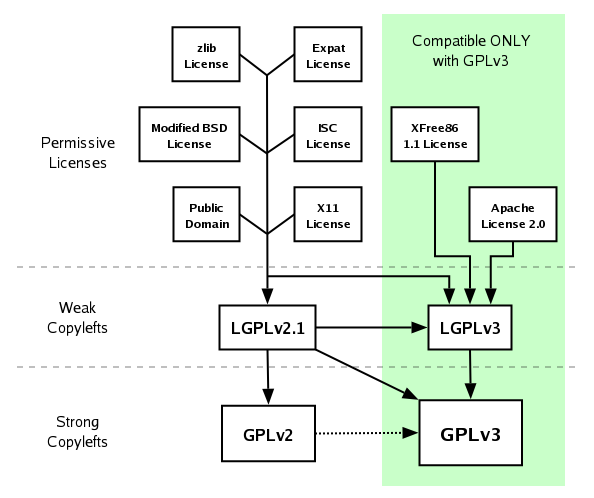
\includegraphics[height=.8\textheight]{compatibility.png}
  
  \small GPL compatibility matrix. Note that GPL 3 is
    GPL 2-incompatible. Figure from \url{http://www.gnu.org/licenses/quick-guide-gplv3.html}.
\end{frame}

\end{document}
